\appendix
\addcontentsline{toc}{chapter}{APPENDIX}
\chapter{\uppercase{Topic 1}}
\section{Logical Errors in Simple Conditional Statements}
\subsection{Switch Case}
In the following algorithm to determine if a character is vowel user had made a typo by entering j instead of i which leads to wrong outputs for both i and j.
\subsubsection{Reference Implementation for Incorrect Branch }
\begin{verbatim}
int isvowel_r(char n) {
    switch(n) {
        case 'a':
            {
                return 1;
                break;
            }
        case 'e':
            {
                return 1;
                break;
            }
        case 'i':
            {
                return 1;
                break;
            }
        case 'o':
            {
                return 1;
                break;
            }
        case 'u':
            {
                return 1;
                break;
            }
        default:
            {
                return 0;
            }
    }              

}
\end{verbatim}
\subsubsection{Error-ridden Implementation for Incorrect Branch}
\begin{verbatim}
int isvowel_i(char n) {
    switch(n) {
        case 'a': 
            {
                return 1;
            }
        case 'e':
            {
                return 1;
            }
        case 'j': 
            {
                return 1;
            }
        case 'o':
            {
                return 1;
            }
        case 'u':
            {
                return 1;
            }

        default:
            {
                return 0;
            }
    }              
}
\end{verbatim}
\subsubsection{Main Function for Incorrect Branch}
\begin{verbatim}
int main(){
    char n;
    klee_make_symbolic(&n, sizeof(n), "n");
    klee_assume(n>='a' && n<='z');
    assert(isvowel_r(n)==isvowel_i(n));
}
\end{verbatim}
\subsubsection{Branch-Appended Reference Implementation for Incorrect Branch}
\begin{verbatim}
int isvowel_r(char n) {
    switch(n) {
        case 'a':
            {
                printf("in branch 5\n");{
                return 1;
                break;
            }
}
        case 'e':
            {
                printf("in branch 4\n");{
                return 1;
                break;
            }
}
        case 'i':
            {
                printf("in branch 3\n");{
                return 1;
                break;
            }
}
        case 'o':
            {
                printf("in branch 2\n");{
                return 1;
                break;
            }
}
        case 'u':
            {
                printf("in branch 1\n");{
                return 1;
                break;
            }
}
        default:
            {
                printf("in branch 0\n");{
                return 0;
            }
}
    }              

}

\end{verbatim}

\subsubsection{Branch-Appended Error-ridden Implementation for Incorrect Branch}
\begin{verbatim}
int isvowel_i(char n) {
    switch(n) {
        case 'a': 
            {
                printf("in branch 11\n");{
                return 1;
            }
}
        case 'e':
            {
                printf("in branch 10\n");{
                return 1;
            }
}
        case 'j': 
            {
                printf("in branch 9\n");{
                return 1;
            }
}
        case 'o':
            {
                printf("in branch 8\n");{
                return 1;
            }
}
        case 'u':
            {
                printf("in branch 7\n");{
                return 1;
            }
}

        default:
            {
                printf("in branch 6\n");{
                return 0;
            }
}
    }              
}
\end{verbatim}
\subsubsection{Result for Incorrect Branch}
\textbf{Input Information}
\begin{verbatim}
object 0: name: 'n'
object 0: size: 1
object 0: data: b'j'
object 0: hex : 0x6a
object 0: int : 106
object 0: uint: 106
object 0: text: j
\end{verbatim}
\textbf{Branches Accessed}
\begin{verbatim}
in branch 0
in branch 9
\end{verbatim}
\begin{figure}[h]
\centering
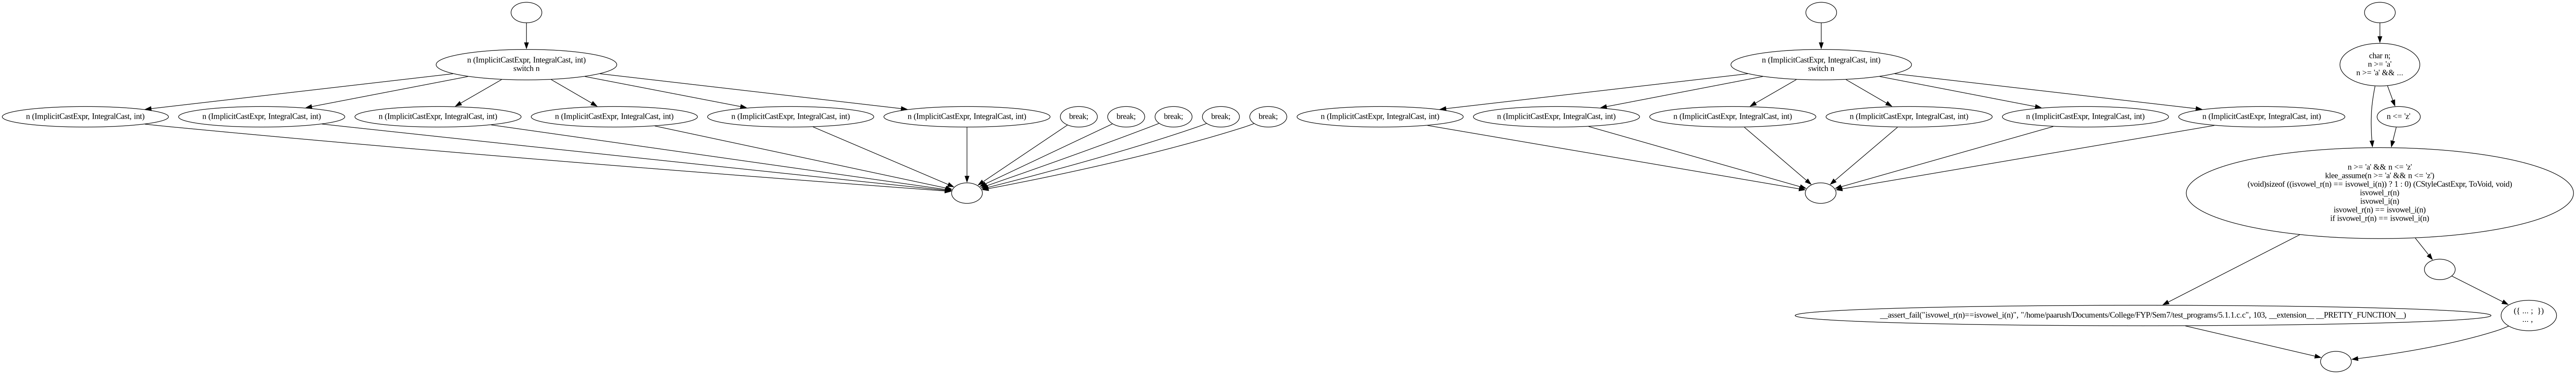
\includegraphics[width=1\textwidth]{5/5.1.1.c.png}
\caption{CFG for Program 5.1.1}
\label{fig:cfg5.1.1}
\end{figure}
\subsubsection{Result Interpretation for Incorrect Branch}
for test case 'j' the switch case takes action corresponding to default case in reference implementation however not so in user implementation hence the user implementation must have falsely classfied as non-default that is vowel case


\section{Logical Errors in Iteration}
For the following examples we take algorithm to determine if a number is prime and introduce logical errors to them as follows and diagonize them.
\subsection{Intialization error}
Here i is intialized from 1 instead of 2 also corner case isn't handled.
\subsubsection{Reference Implementation for Loop Start Error}
\begin{verbatim}
int isPrime_r(int n)
{
    // Corner case
    if (n <= 1)
        return 0;
    // Check from 2 to square root of n
    for (int i = 2; i <= n-1; i++)
        if (n % i == 0)
            return 0;
    return 1;
}
\end{verbatim}
\subsubsection{Error-ridden Implementation for Loop Start Error}
\begin{verbatim}
int isPrime_i(int n)
{
    if (n <= 1)
        return 0;
    // Check from 2 to square root of n
    for (int i = 1; i <= n-1; i++)
        if (n % i == 0)
            return 0;
    return 1;
}
\end{verbatim}
\subsubsection{Main Function for Loop Start Error}
\begin{verbatim}
int main(){
    int n;
    klee_make_symbolic(&n, sizeof(n), "n");
    klee_assume(n>=0 && n<=10);
    assert(isPrime_r(n)==isPrime_i(n));
}
\end{verbatim}
\subsubsection{Branch-Appended Reference Implementation for Loop Start Error}

\begin{verbatim}
int isPrime_r(int n)
{
    // Corner case
    if (n <= 1)
        {
            printf("in branch 0\n");return 0;}

    // Check from 2 to square root of n
    for (int i = 2; i <= n-1; i++)
        {
            printf("in branch 1\n");if (n % i == 0)
            {
                printf("in branch 2\n");return 0;}}

    return 1;
}
\end{verbatim}

\subsubsection{Branch-Appended Error-ridden Implementation for Loop Start Error}

\begin{verbatim}
int isPrime_i(int n)
{
    // Corner case
    if (n <= 1)
        {
            printf("in branch 3\n");return 0;}

    // Check from 2 to square root of n
    for (int i = 1; i <= n-1; i++)
        {
            printf("in branch 4\n");if (n % i == 0)
            {
                printf("in branch 5\n");return 0;}}
    return 1;
}
\end{verbatim}
\subsubsection{Result for Loop Start Error}
\textbf{Input Information}
\begin{verbatim}
object 0: name: 'n'
object 0: size: 4
object 0: data: b'\x02\x00\x00\x00'
object 0: hex : 0x02000000
object 0: int : 2
object 0: uint: 2
object 0: text: ....
\end{verbatim}


\textbf{Branches Accessed}
\begin{verbatim}
in branch 4
in branch 5
\end{verbatim}
\begin{figure}[h]
\centering
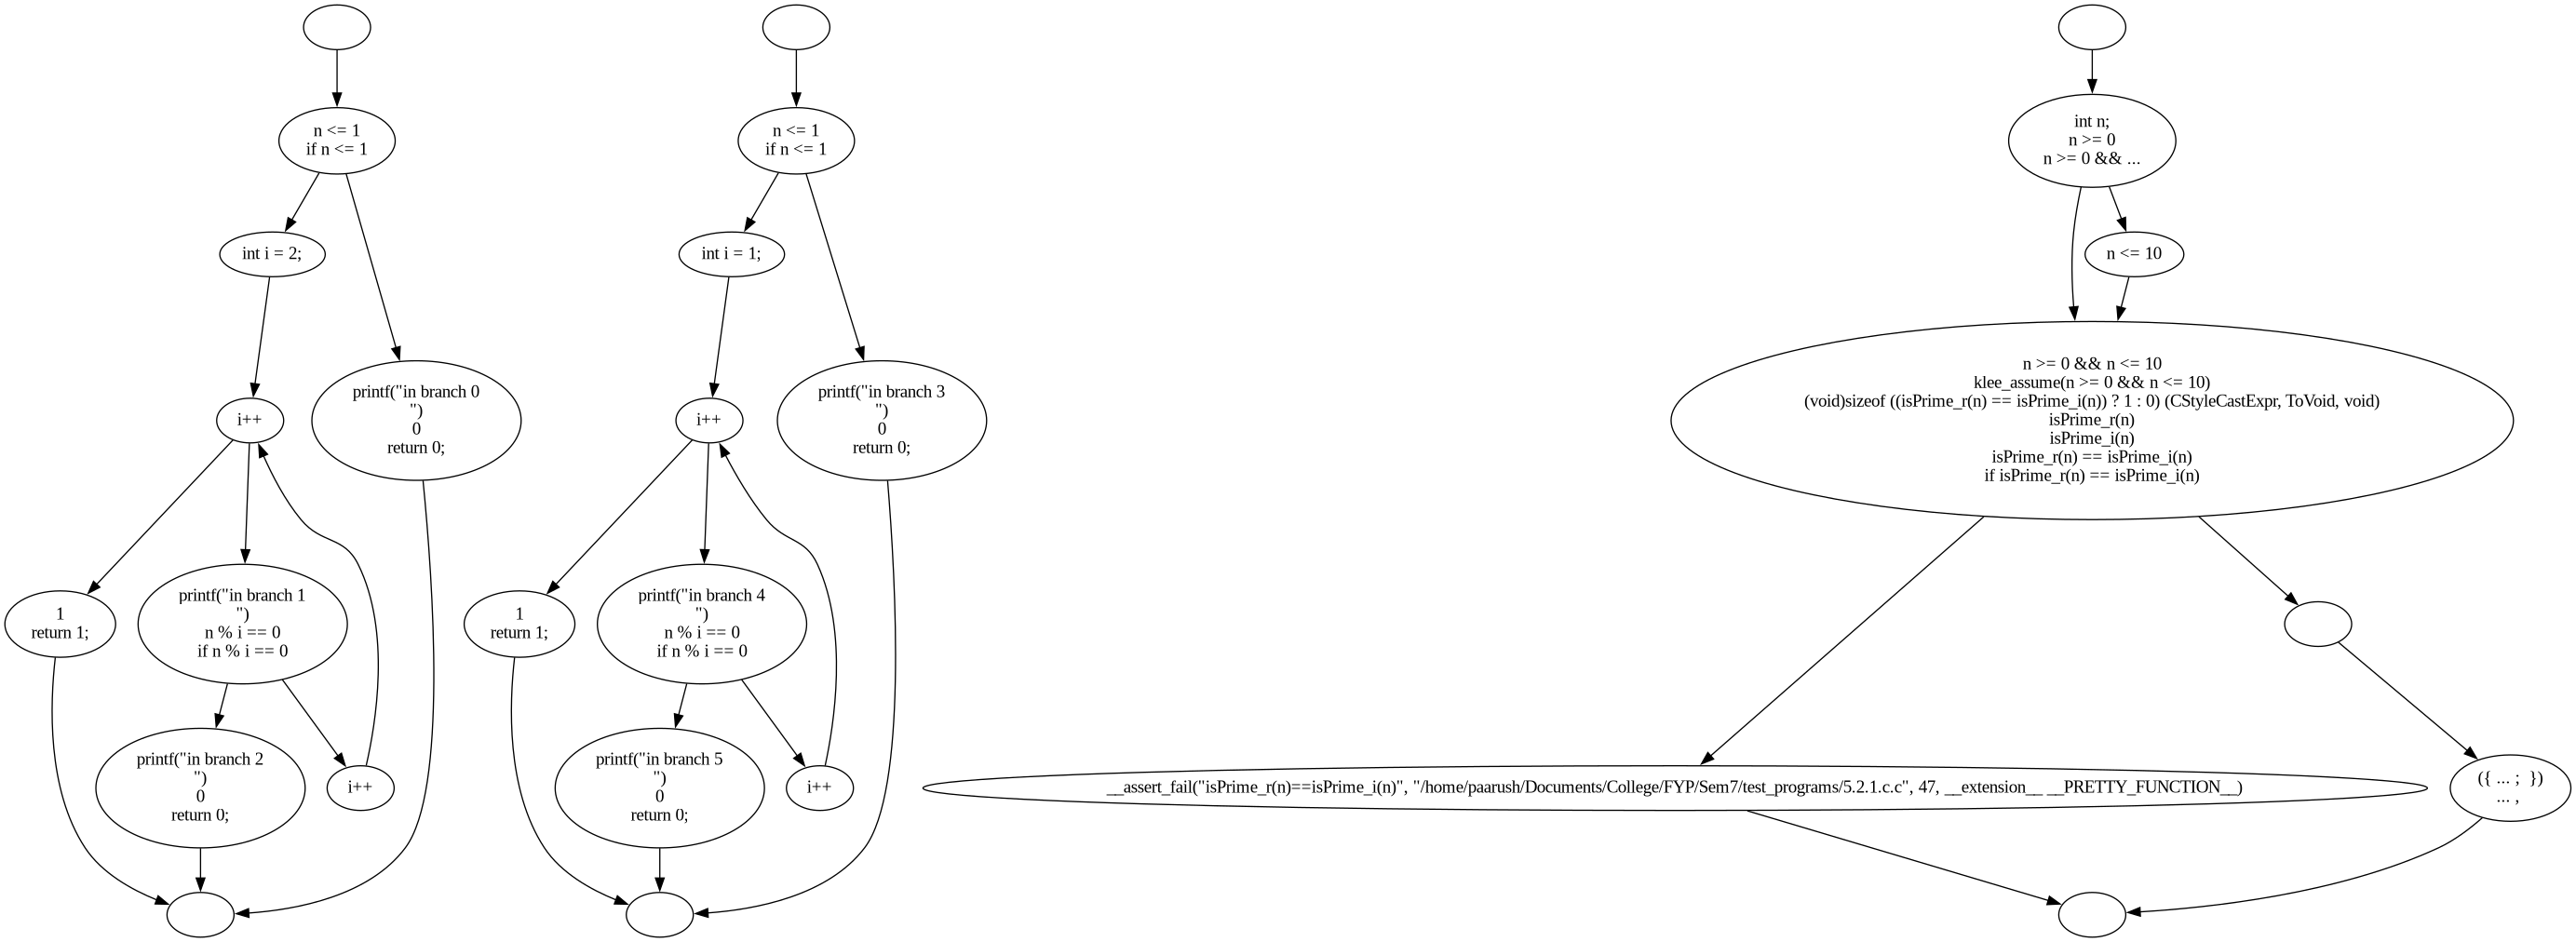
\includegraphics[width=1\textwidth]{5/5.2.1.c.png}
\caption{CFG for Program 5.2.1}
\label{fig:cfg5.2.1}
\end{figure}
\subsubsection{Result Interpretation for Loop Start Error}
for test case value 2 the user implementation had entered branch 4 but reference implementation had not entered branch 2 hence it can be attributed to entry condition error.
\subsection{Termination error}
Here termination is supposed to be $i<=n-1$ however we terminate at $i<=n$
\subsubsection{Reference Implementation for Loop End Error}
\begin{verbatim}
int isPrime_r(int n)
{
    // Corner case
    if (n <= 1)
        return false;
 
    // Check from 2 to square root of n
    for (int i = 2; i <= n-1; i++)
        if (n % i == 0)
            return false;
 
    return true;
}
\end{verbatim}
\subsubsection{Error-ridden Implementation for Loop End Error}
\begin{verbatim}
int isPrime_i(int n)
{
    // Check from 2 to square root of n
    if (n <= 1)
		return 0;
    for (int i = 2; i <= n; i++)
        if (n % i == 0)
            return false;
    return true;
}
\end{verbatim}
\subsubsection{Main Function for Loop End Error}
\begin{verbatim}
int main(){
    int n;
    klee_make_symbolic(&n, sizeof(n), "n");
    klee_assume(n>=0 && n<=10);
    assert(isPrime_r(n)==isPrime_i(n));
}
\end{verbatim}
\subsubsection{Branch-Appended Reference Implementation for Loop End Error}
\begin{verbatim}
int isPrime_r(int n)
{
    // Corner case
    if (n <= 1)
        {
            printf("in branch 0\n");return 0;}

    // Check from 2 to square root of n
    for (int i = 2; i <= n-1; i++)
        {
            printf("in branch 1\n");if (n % i == 0)
            {
                printf("in branch 2\n");return 0;}}

    return 1;
}
\end{verbatim}

\subsubsection{Branch-Appended Error-ridden Implementation for Loop End Error}

\begin{verbatim}
int isPrime_i(int n)
{
    // Corner case
    if (n <= 1)
        {
            printf("in branch 3\n");return 0;}

    // Check from 2 to square root of n
    for (int i = 2; i <= n; i++)
        {
            printf("in branch 4\n");if (n % i == 0)
            {
                printf("in branch 5\n");return 0;}}
    return 1;
}
\end{verbatim}
\subsubsection{Result for Loop End Error}
\textbf{Input Information}
\begin{verbatim}
object 0: name: 'n'
object 0: size: 4
object 0: data: b'\x02\x00\x00\x00'
object 0: hex : 0x02000000
object 0: int : 2
object 0: uint: 2
object 0: text: ....
\end{verbatim}
\textbf{Branches Accessed}
\begin{verbatim}
in branch 4
in branch 5
\end{verbatim}
\begin{figure}[h]
\centering
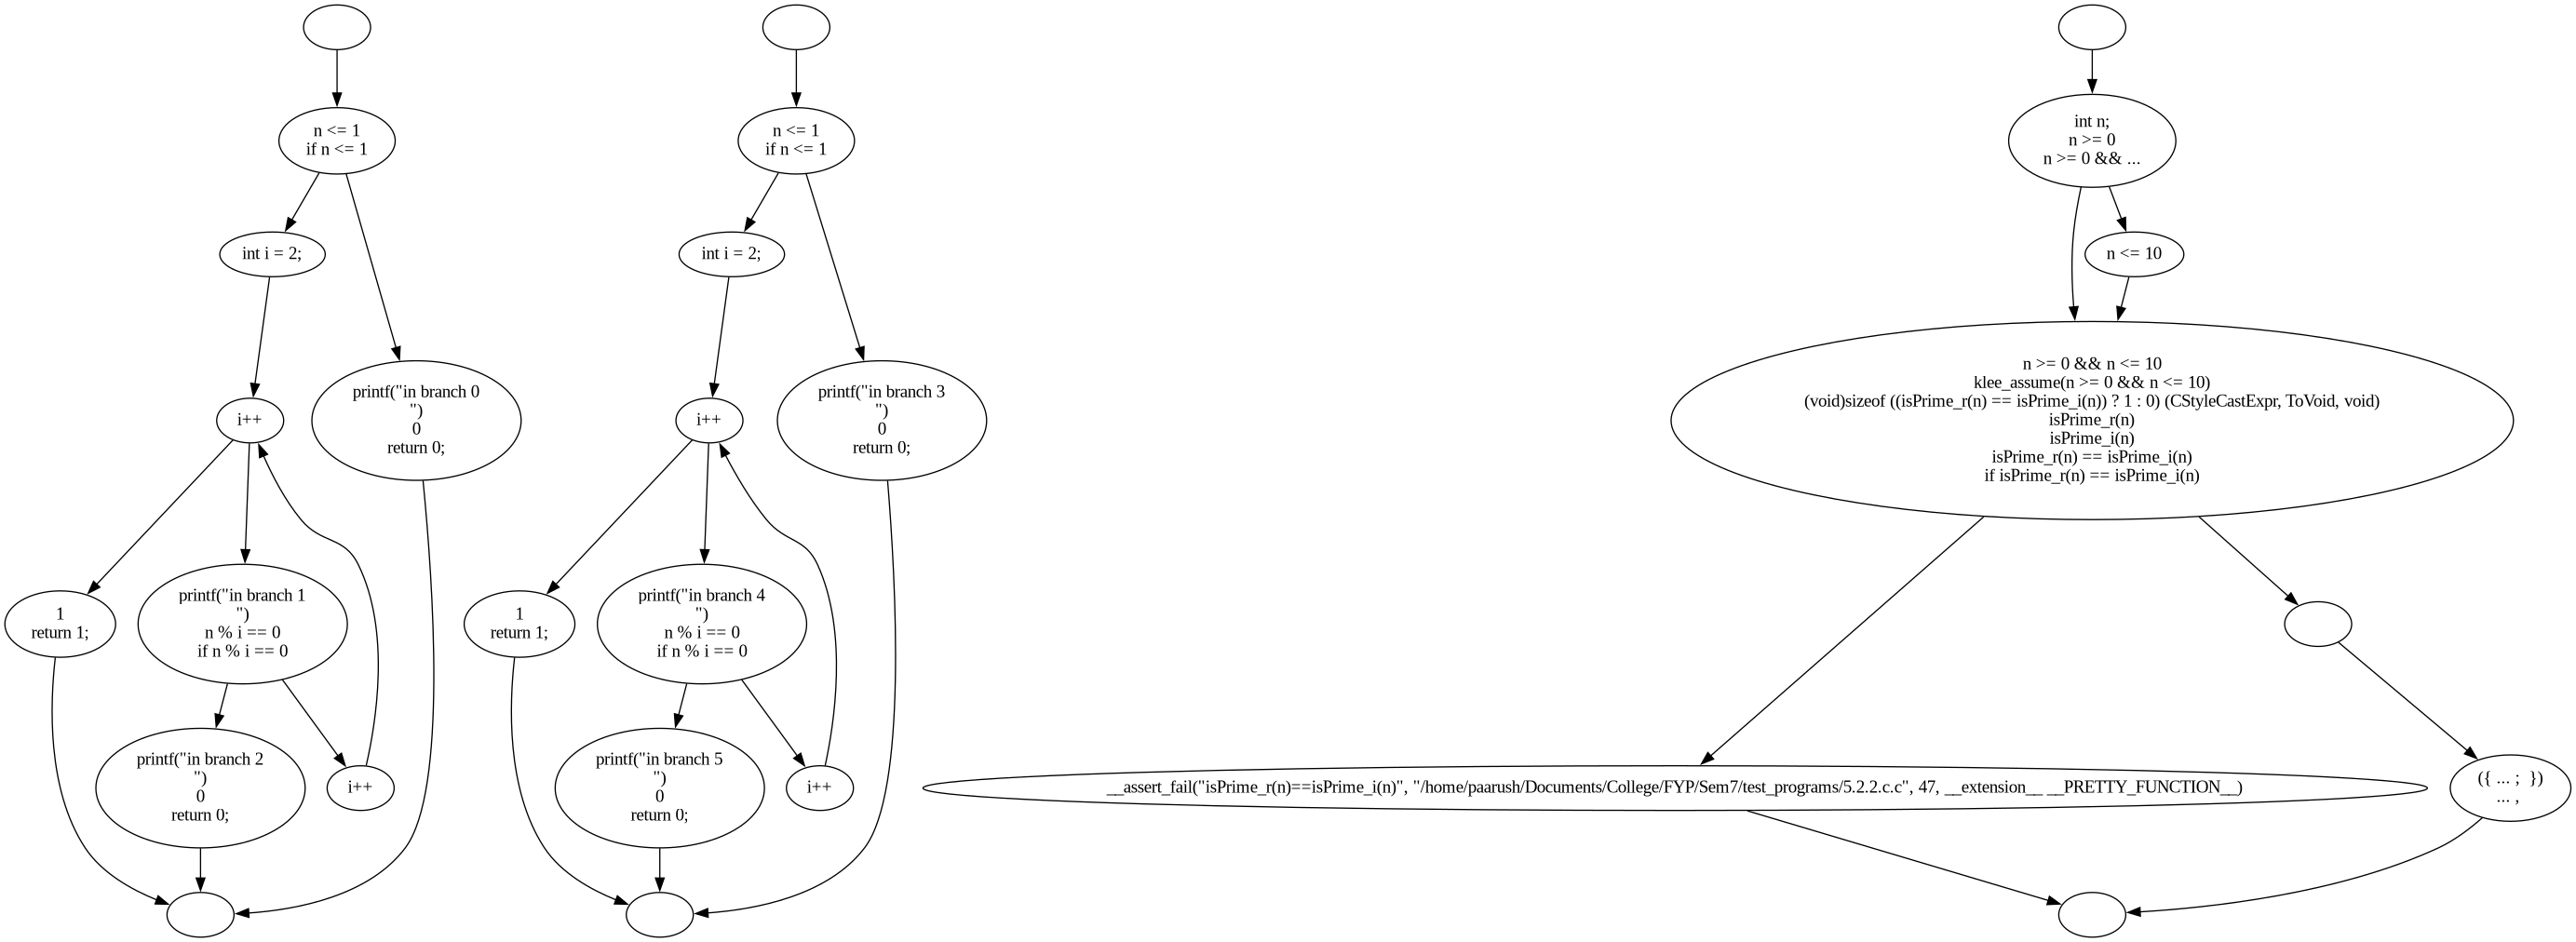
\includegraphics[width=1\textwidth]{5/5.2.2.c.png}
\caption{CFG for Program 5.2.2}
\label{fig:cfg5.2.2}
\end{figure}
\subsubsection{Result Interpretation for Loop End Error}
Here wrong termination condition has failed test case- 2 as 2 enters into branch 4 so it must have staisfied termination constraint hence error can be attributed to it.



\subsection{Control variable updation error}
Here control variable is updated as i+=2 instead of i+=1
\subsubsection{Reference Implementation for Loop Increment Error}
\begin{verbatim}
bool isPrime_r(int n)
{
    // Corner case
    if (n <= 1)
        return false;
 
    // Check from 2 to square root of n
    for (int i = 2; i <= n-1; i++)
        if (n % i == 0)
            return false;
 
    return true;
}
\end{verbatim}
\subsubsection{Error-ridden Implementation for Loop Increment Error}
\begin{verbatim}
bool isPrime_i(int n)
{
    // Corner case
      if (n <= 1)
        return false;
 
    // Check from 2 to square root of n
    for (int i = 2; i <= n-1;i+=2 )
        if (n % i == 0)
            return false;
 
    return true;
}
\end{verbatim}
\subsubsection{Main Function for Loop Increment Error}
\begin{verbatim}
int main(){
    int n;
    klee_make_symbolic(&n, sizeof(n), "n");
    klee_assume(n>=0 && n<=10);
    assert(isPrime_r(n)==isPrime_i(n));
}
\end{verbatim}
\subsubsection{Branch-Appended Reference Implementation for Loop Increment Error}
\begin{verbatim}
int isPrime_r(int n)
{
    // Corner case
    if (n <= 1)
        {
            printf("in branch 0\n");return 0;}

    // Check from 2 to square root of n
    for (int i = 2; i <= n-1; i++)
        {
            printf("in branch 1\n");if (n % i == 0)
            {
                printf("in branch 2\n");return 0;}}

    return 1;
}
\end{verbatim}

\subsubsection{Branch-Appended Error-ridden Implementation for Loop Increment Error}

\begin{verbatim}
int isPrime_i(int n)
{
    // Corner case
    if (n <= 1)
        {
            printf("in branch 3\n");return 0;}

    // Check from 2 to square root of n
    for (int i = 2; i <= n-1; i+=2)
        {
            printf("in branch 4\n");if (n % i == 0)
            {
                printf("in branch 5\n");return 0;}}

    return 1;
}
\end{verbatim}
\subsubsection{Result for Loop Increment Error}
\textbf{Input Information}
\begin{verbatim}
object 0: name: 'n'
object 0: size: 4
object 0: data: b'\t\x00\x00\x00'
object 0: hex : 0x09000000
object 0: int : 9
object 0: uint: 9
object 0: text: ....
\end{verbatim}
\textbf{Branches Accessed}
\begin{verbatim}
in branch 1
in branch 1
in branch 2
in branch 4
in branch 4
in branch 4
in branch 4
\end{verbatim}
\begin{figure}[h]
\centering
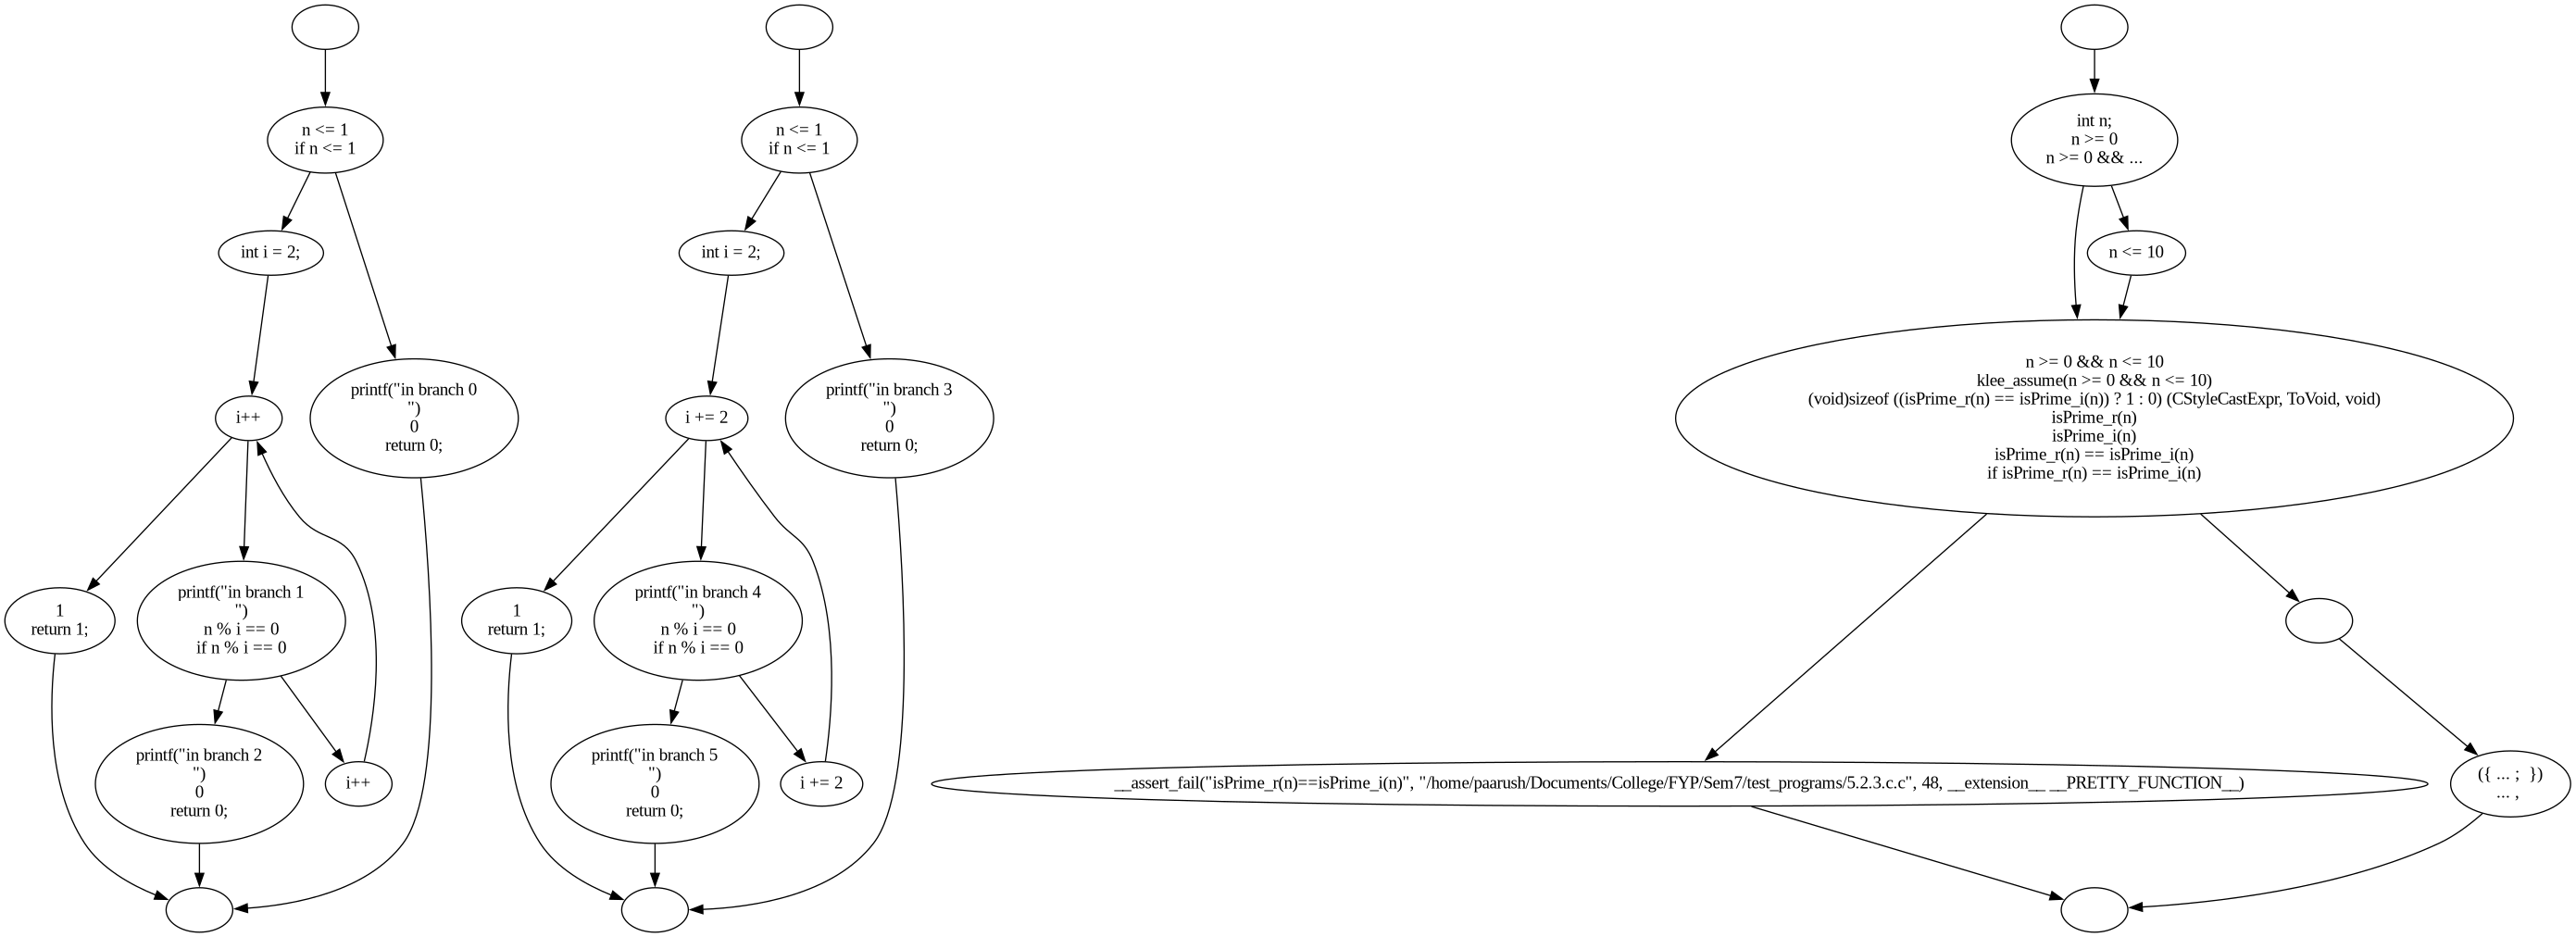
\includegraphics[width=1\textwidth]{5/5.2.3.c.png}
\caption{CFG for Program 5.2.3}
\label{fig:cfg5.2.3}
\end{figure}
\subsubsection{Result Interpretation for Loop Increment Error}
The loop in the reference implementation has run 2 times and on the second run, it has entered branch 2.
The loop in the error implementation has run 4 times and not entered branch 5. This suggests that the loop has completed without reaching the factor. This would mean the factor was skipped and likely is an issue with the increment operator in the for loop.

\subsection{Infinite Loop}
Here incorrect/negligence of termination statement leads to infinite loop
\subsubsection{Reference Implementation for Infinite Loop Error}
\begin{verbatim}
int isPrime_r(int n)
{
    // Corner case
    if (n <= 1)
        return 0;

    // Check from 2 to square root of n
    for (int i = 2; i <= n-1; i++)
        if (n % i == 0)
            return 0;

    return 1;
}
\end{verbatim}
\subsubsection{Error-ridden Implementation for Infinite Loop Error}
\begin{verbatim}
int isPrime_i(int n)
{
    // Corner case
    if (n <= 1)
        return 0;

    // Check from 2 to square root of n
    for (int i = 2; i <= n-1;)
        if (n % i == 0)
            return 0;

    return 1;
}

\end{verbatim}

\subsubsection{Main Function for Infinite Loop Error}
\begin{verbatim}
int main(){
    int n;
    klee_make_symbolic(&n, sizeof(n), "n");
    klee_assume(n>=0 && n<=10);
    assert(isPrime_r(n)==isPrime_i(n));
}
\end{verbatim}
\subsubsection{Branch-Appended Reference Implementation for Infinite Loop Error}
\begin{verbatim}
int isPrime_r(int n)
{
    // Corner case
    if (n <= 1)
        {
            printf("in branch 0\n");return 0;}

    // Check from 2 to square root of n
    for (int i = 2; i <= n-1; i++)
        {
            printf("in branch 1\n");if (n % i == 0)
            {
                printf("in branch 2\n");return 0;}}

    return 1;
}
\end{verbatim}

\subsubsection{Branch-Appended Error-ridden Implementation for Infinite Loop Error}

\begin{verbatim}
int isPrime_i(int n)
{
    // Corner case
    if (n <= 1)
        {
            printf("in branch 3\n");return 0;}

    // Check from 2 to square root of n
    for (int i = 2; i <= n-1; )
        {
            printf("in branch 4\n");if (n % i == 0)
            {
                printf("in branch 5\n");return 0;}}

    return 1;
}
\end{verbatim}
\subsubsection{Result for Infinite Loop Error}
\textbf{Input Information}
\begin{verbatim}
object 0: name: 'n'
object 0: size: 4
object 0: data: b'\t\x00\x00\x00'
object 0: hex : 0x09000000
object 0: int : 9
object 0: uint: 9
object 0: text: ....
\end{verbatim}
\textbf{Branches Accessed}
\begin{verbatim}
in branch 1
in branch 1
in branch 2
in branch 4
in branch 4
in branch 4
in branch 4
...
\end{verbatim}
\begin{figure}[h]
\centering
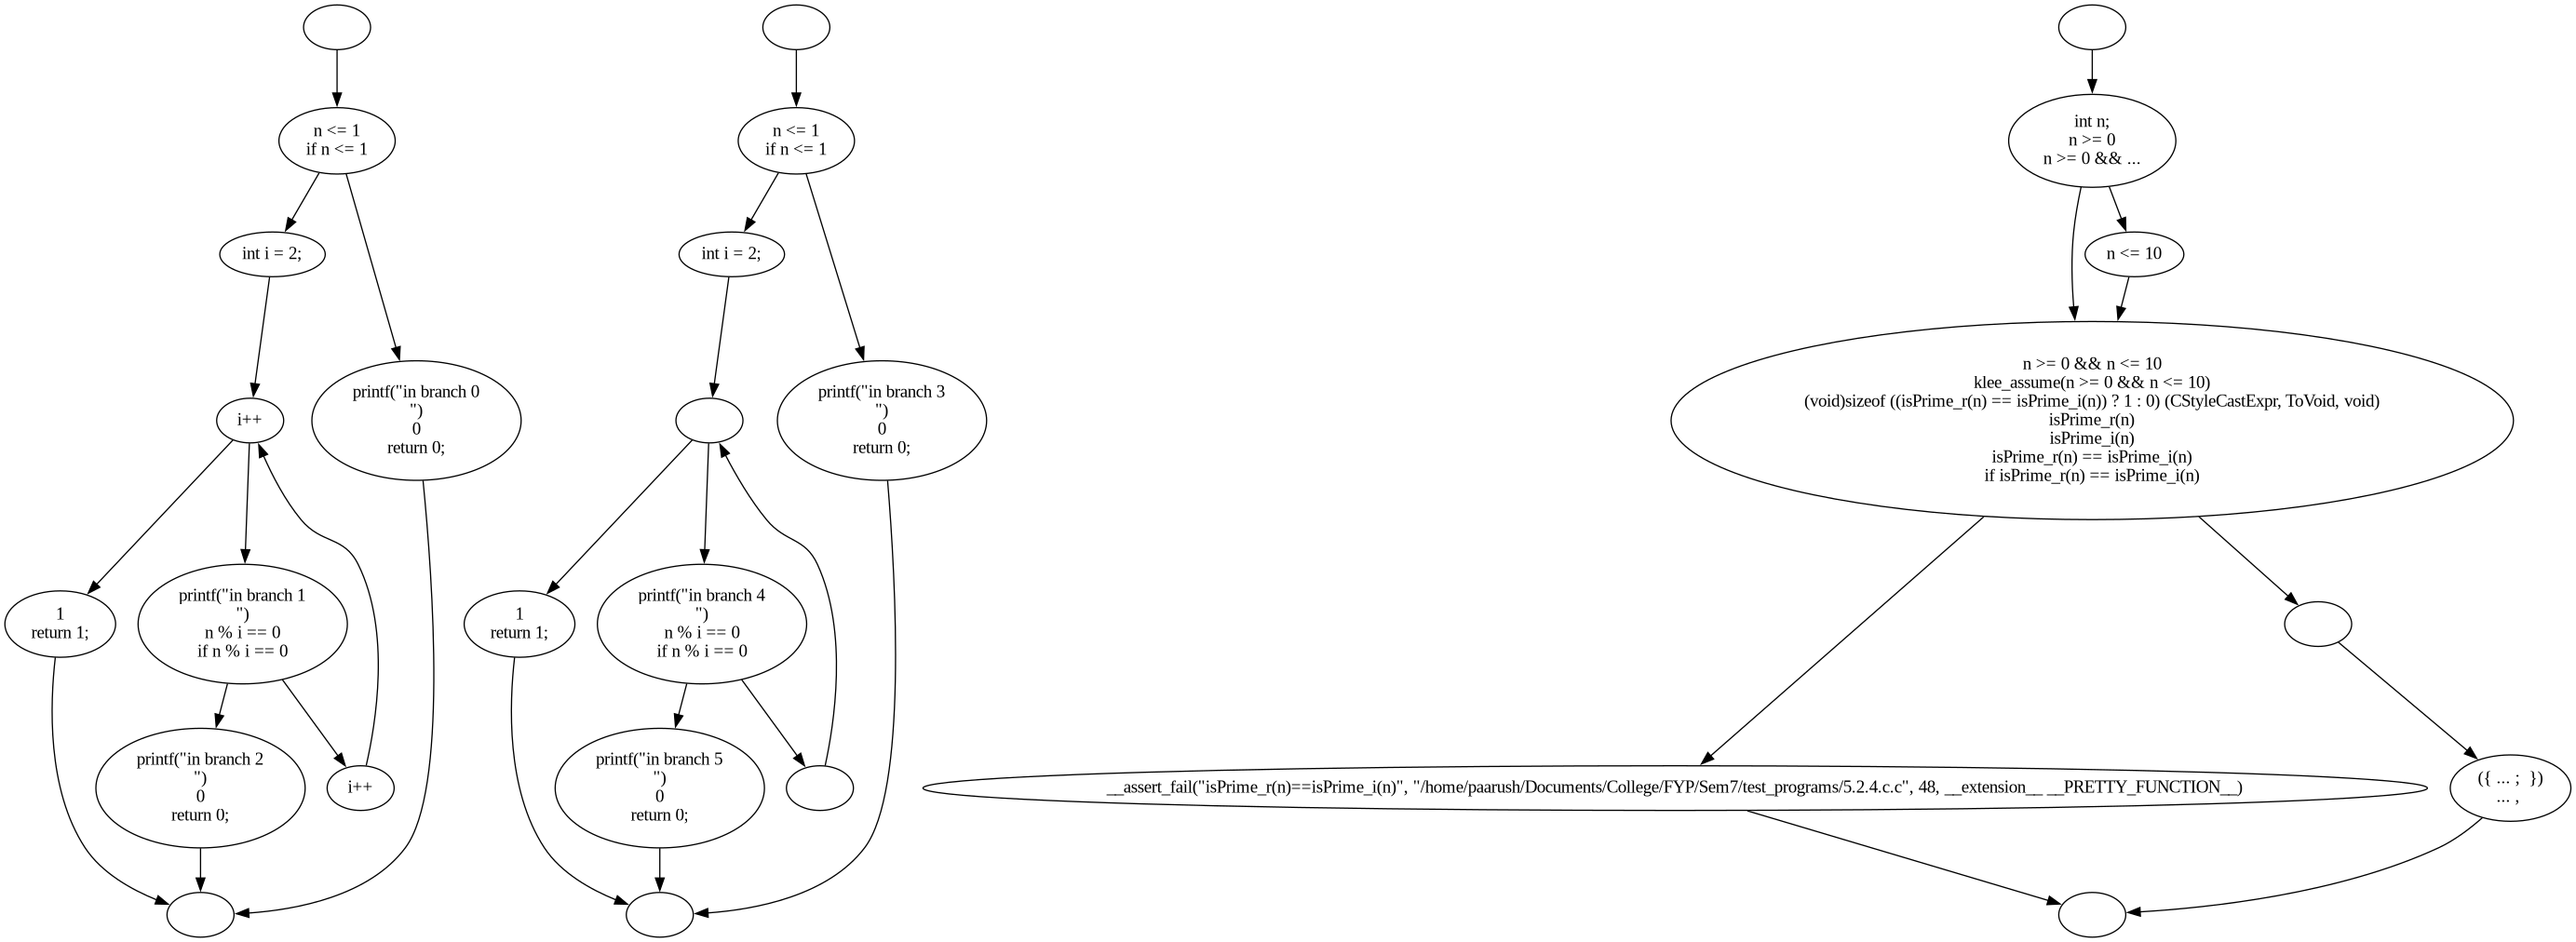
\includegraphics[width=1\textwidth]{5/5.2.4.c.png}
\caption{CFG for Program 5.2.4}
\label{fig:cfg5.2.4}
\end{figure}
\subsubsection{Result Interpretation for Infinite Loop Error}
Here we can notice branch 4 repeatedly visited hence there must be infinite loop in the code.


\section{Logical Errors in Recursion}
\subsection{Errors in Recurrence Relation for Incorrect Recursion Error}
Here error is made in recurrence relation 
$f(x)=f(x-2)+f(x-2)$ instead of $f(x)=f(x-1)+f(x-2)$.
\subsubsection{Reference Implementation for Incorrect Recursion Error}
\begin{verbatim}
int fib_r(int x){
    if (x==0) {
        return 0;
    } else if(x==1){
        return 1;
    }
    else {
        return fib_r(x-2)+fib_r(x-2);
    }
}
\end{verbatim}
\subsubsection{Error-ridden Implementation for Incorrect Recursion Error}
\begin{verbatim}
int fib_i(int x){
    if(x==0) {
        return 0;
    } else if(x==1) {
        return 1;
    } else {
        return fib_i(x-1)+fib_i(x-2);
    }
}
\end{verbatim}
\subsubsection{Main Function for Incorrect Recursion Error}
\begin{verbatim}
int main(){
    int x;
    klee_make_symbolic(&x, sizeof(x), "x");
    klee_assume(x>=0 && x<=5);
    assert(fib_i(x)==fib_r(x));
}
\end{verbatim}
\subsubsection{Branch-Appended Error-ridden Implementation for Incorrect Recursion Error}
\begin{verbatim}
int fib_r(int x){
    if (x==0) {
        printf("in branch 0\n");{
        return 0;
    } }else {
        printf("in branch 1\n");if(x==1){
        printf("in branch 2\n");{
        return 1;
    }
} else {
        printf("in branch 3\n");{
        return fib_r(x-2)+fib_r(x-2);
    }
}}}
\end{verbatim}

\subsubsection{Branch-Appended Reference Implementation for Incorrect Recursion Error}

\begin{verbatim}
int fib_i(int x){
    if(x==0) {
        printf("in branch 4\n");{
        return 0;
    } }else {
        printf("in branch 5\n");if(x==1) {
        printf("in branch 6\n");{
        return 1;
    } }else {
        printf("in branch 7\n");{
        return fib_i(x-1)+fib_i(x-2);
    }
}}}
\end{verbatim}

\subsubsection{Result for Incorrect Recursion Error}
\textbf{Input Information}
\begin{verbatim}
object 0: name: 'x'
object 0: size: 4
object 0: data: b'\x02\x00\x00\x00'
object 0: hex : 0x02000000
object 0: int : 2
object 0: uint: 2
object 0: text: .... 
\end{verbatim}
\textbf{Branches Accessed}
\begin{verbatim}
in branch 5
in branch 7
in branch 5
in branch 6
in branch 4
in branch 1
in branch 3
in branch 0
in branch 0
\end{verbatim}
\begin{figure}[h]
\centering
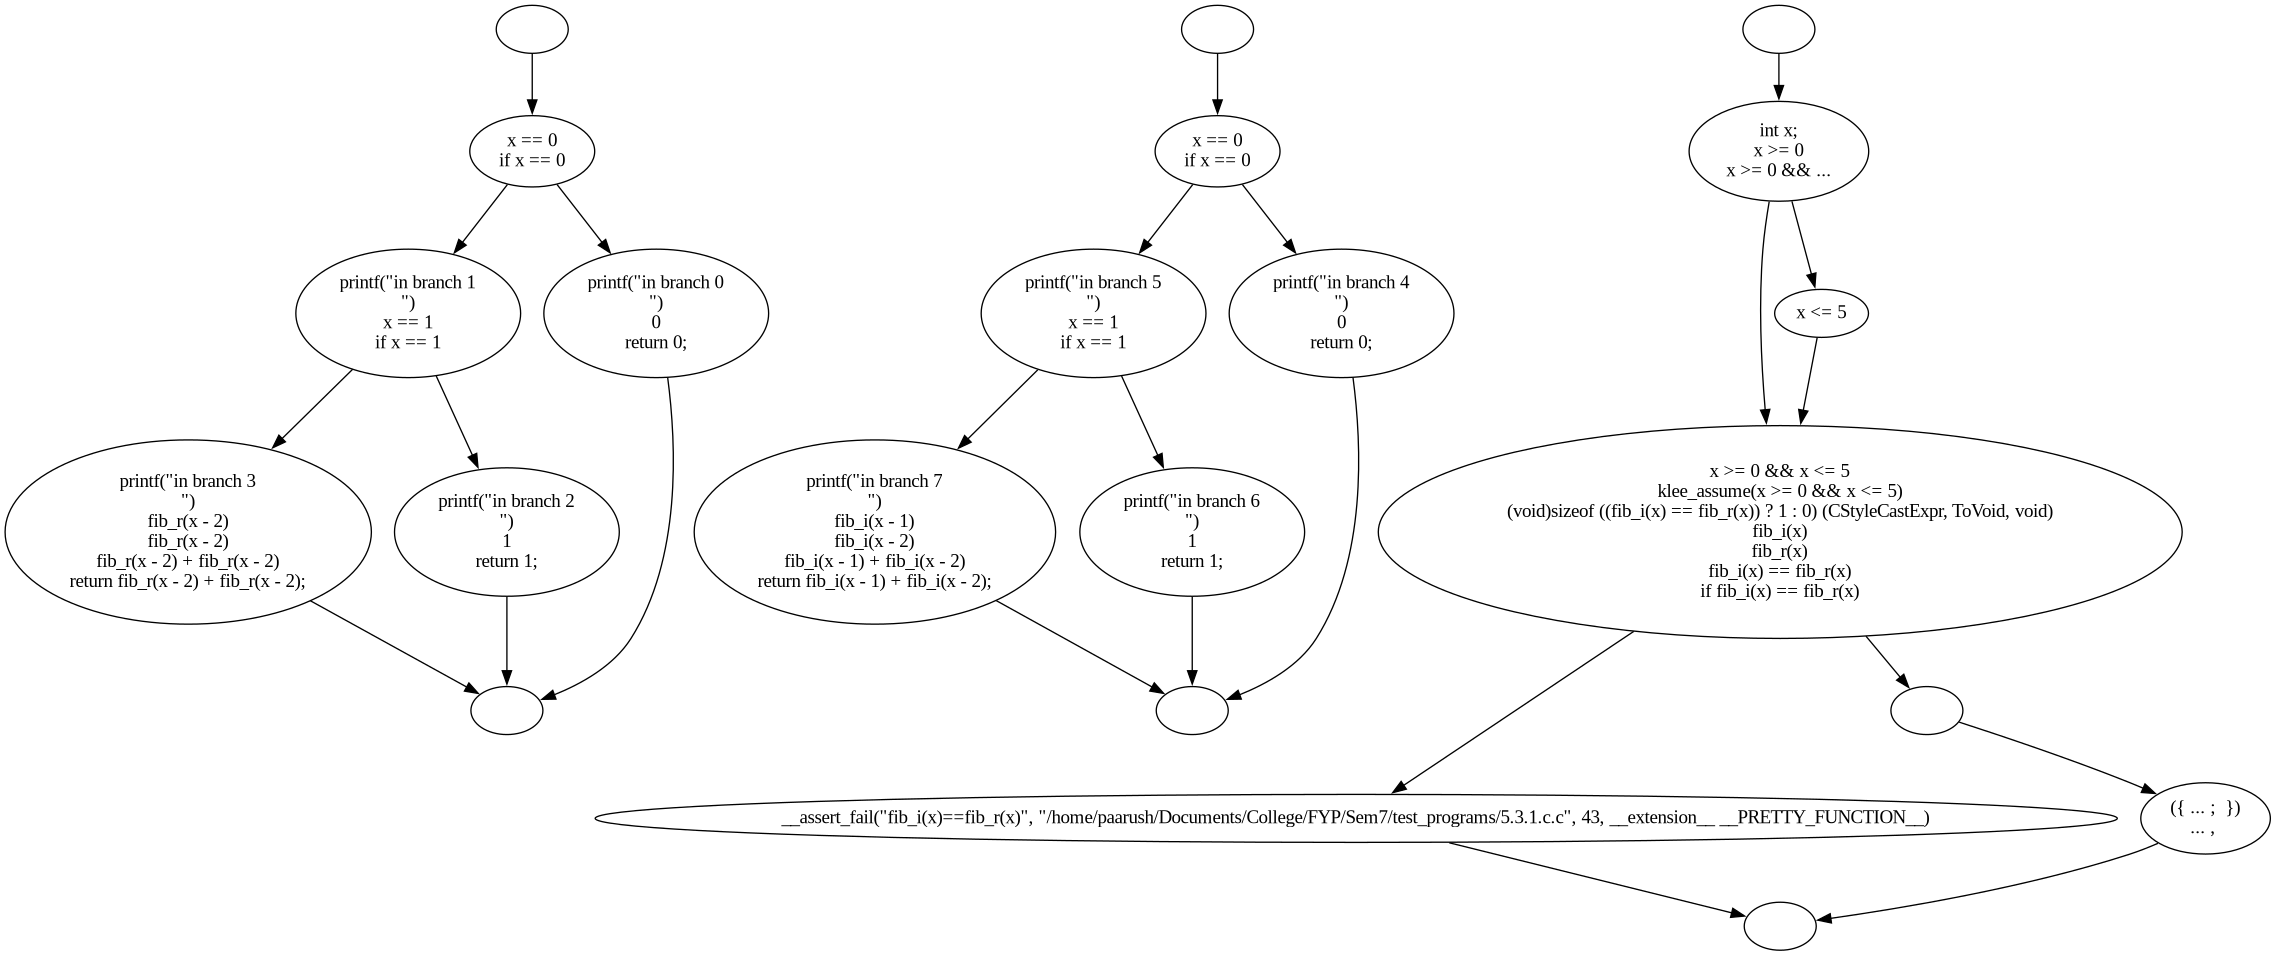
\includegraphics[width=1\textwidth]{5/5.3.1.c.png}
\caption{CFG for Program 5.3.1}
\label{fig:cfg5.3.1}
\end{figure}
\subsubsection{Result Interpretation for Incorrect Recursion Error}
Looking at the similarity in structure of branches correspondence 3-7,1-5,2-6,0-4 can be established  where 0 to 3 belong to user and 4 to 7 belong to reference implementation.
by analyzing patter 5,7,5,6,4 becomes 1,3,1,2,0 which is very different from 1,3,0,0 hence the entire recurrence relation could be attributed to cause of error furthermore 0,0 reflects same branch taken which isn't an expected behaviour from the program




